\documentclass[]{article}
\usepackage{lmodern}
\usepackage{amssymb,amsmath}
\usepackage{ifxetex,ifluatex}
\usepackage{fixltx2e} % provides \textsubscript
\ifnum 0\ifxetex 1\fi\ifluatex 1\fi=0 % if pdftex
  \usepackage[T1]{fontenc}
  \usepackage[utf8]{inputenc}
\else % if luatex or xelatex
  \ifxetex
    \usepackage{mathspec}
  \else
    \usepackage{fontspec}
  \fi
  \defaultfontfeatures{Ligatures=TeX,Scale=MatchLowercase}
\fi
% use upquote if available, for straight quotes in verbatim environments
\IfFileExists{upquote.sty}{\usepackage{upquote}}{}
% use microtype if available
\IfFileExists{microtype.sty}{%
\usepackage{microtype}
\UseMicrotypeSet[protrusion]{basicmath} % disable protrusion for tt fonts
}{}
\usepackage[margin=1in]{geometry}
\usepackage{hyperref}
\hypersetup{unicode=true,
            pdftitle={FinalReport},
            pdfauthor={cyber-atlas},
            pdfborder={0 0 0},
            breaklinks=true}
\urlstyle{same}  % don't use monospace font for urls
\usepackage{color}
\usepackage{fancyvrb}
\newcommand{\VerbBar}{|}
\newcommand{\VERB}{\Verb[commandchars=\\\{\}]}
\DefineVerbatimEnvironment{Highlighting}{Verbatim}{commandchars=\\\{\}}
% Add ',fontsize=\small' for more characters per line
\usepackage{framed}
\definecolor{shadecolor}{RGB}{248,248,248}
\newenvironment{Shaded}{\begin{snugshade}}{\end{snugshade}}
\newcommand{\AlertTok}[1]{\textcolor[rgb]{0.94,0.16,0.16}{#1}}
\newcommand{\AnnotationTok}[1]{\textcolor[rgb]{0.56,0.35,0.01}{\textbf{\textit{#1}}}}
\newcommand{\AttributeTok}[1]{\textcolor[rgb]{0.77,0.63,0.00}{#1}}
\newcommand{\BaseNTok}[1]{\textcolor[rgb]{0.00,0.00,0.81}{#1}}
\newcommand{\BuiltInTok}[1]{#1}
\newcommand{\CharTok}[1]{\textcolor[rgb]{0.31,0.60,0.02}{#1}}
\newcommand{\CommentTok}[1]{\textcolor[rgb]{0.56,0.35,0.01}{\textit{#1}}}
\newcommand{\CommentVarTok}[1]{\textcolor[rgb]{0.56,0.35,0.01}{\textbf{\textit{#1}}}}
\newcommand{\ConstantTok}[1]{\textcolor[rgb]{0.00,0.00,0.00}{#1}}
\newcommand{\ControlFlowTok}[1]{\textcolor[rgb]{0.13,0.29,0.53}{\textbf{#1}}}
\newcommand{\DataTypeTok}[1]{\textcolor[rgb]{0.13,0.29,0.53}{#1}}
\newcommand{\DecValTok}[1]{\textcolor[rgb]{0.00,0.00,0.81}{#1}}
\newcommand{\DocumentationTok}[1]{\textcolor[rgb]{0.56,0.35,0.01}{\textbf{\textit{#1}}}}
\newcommand{\ErrorTok}[1]{\textcolor[rgb]{0.64,0.00,0.00}{\textbf{#1}}}
\newcommand{\ExtensionTok}[1]{#1}
\newcommand{\FloatTok}[1]{\textcolor[rgb]{0.00,0.00,0.81}{#1}}
\newcommand{\FunctionTok}[1]{\textcolor[rgb]{0.00,0.00,0.00}{#1}}
\newcommand{\ImportTok}[1]{#1}
\newcommand{\InformationTok}[1]{\textcolor[rgb]{0.56,0.35,0.01}{\textbf{\textit{#1}}}}
\newcommand{\KeywordTok}[1]{\textcolor[rgb]{0.13,0.29,0.53}{\textbf{#1}}}
\newcommand{\NormalTok}[1]{#1}
\newcommand{\OperatorTok}[1]{\textcolor[rgb]{0.81,0.36,0.00}{\textbf{#1}}}
\newcommand{\OtherTok}[1]{\textcolor[rgb]{0.56,0.35,0.01}{#1}}
\newcommand{\PreprocessorTok}[1]{\textcolor[rgb]{0.56,0.35,0.01}{\textit{#1}}}
\newcommand{\RegionMarkerTok}[1]{#1}
\newcommand{\SpecialCharTok}[1]{\textcolor[rgb]{0.00,0.00,0.00}{#1}}
\newcommand{\SpecialStringTok}[1]{\textcolor[rgb]{0.31,0.60,0.02}{#1}}
\newcommand{\StringTok}[1]{\textcolor[rgb]{0.31,0.60,0.02}{#1}}
\newcommand{\VariableTok}[1]{\textcolor[rgb]{0.00,0.00,0.00}{#1}}
\newcommand{\VerbatimStringTok}[1]{\textcolor[rgb]{0.31,0.60,0.02}{#1}}
\newcommand{\WarningTok}[1]{\textcolor[rgb]{0.56,0.35,0.01}{\textbf{\textit{#1}}}}
\usepackage{graphicx,grffile}
\makeatletter
\def\maxwidth{\ifdim\Gin@nat@width>\linewidth\linewidth\else\Gin@nat@width\fi}
\def\maxheight{\ifdim\Gin@nat@height>\textheight\textheight\else\Gin@nat@height\fi}
\makeatother
% Scale images if necessary, so that they will not overflow the page
% margins by default, and it is still possible to overwrite the defaults
% using explicit options in \includegraphics[width, height, ...]{}
\setkeys{Gin}{width=\maxwidth,height=\maxheight,keepaspectratio}
\IfFileExists{parskip.sty}{%
\usepackage{parskip}
}{% else
\setlength{\parindent}{0pt}
\setlength{\parskip}{6pt plus 2pt minus 1pt}
}
\setlength{\emergencystretch}{3em}  % prevent overfull lines
\providecommand{\tightlist}{%
  \setlength{\itemsep}{0pt}\setlength{\parskip}{0pt}}
\setcounter{secnumdepth}{0}
% Redefines (sub)paragraphs to behave more like sections
\ifx\paragraph\undefined\else
\let\oldparagraph\paragraph
\renewcommand{\paragraph}[1]{\oldparagraph{#1}\mbox{}}
\fi
\ifx\subparagraph\undefined\else
\let\oldsubparagraph\subparagraph
\renewcommand{\subparagraph}[1]{\oldsubparagraph{#1}\mbox{}}
\fi

%%% Use protect on footnotes to avoid problems with footnotes in titles
\let\rmarkdownfootnote\footnote%
\def\footnote{\protect\rmarkdownfootnote}

%%% Change title format to be more compact
\usepackage{titling}

% Create subtitle command for use in maketitle
\providecommand{\subtitle}[1]{
  \posttitle{
    \begin{center}\large#1\end{center}
    }
}

\setlength{\droptitle}{-2em}

  \title{FinalReport}
    \pretitle{\vspace{\droptitle}\centering\huge}
  \posttitle{\par}
    \author{cyber-atlas}
    \preauthor{\centering\large\emph}
  \postauthor{\par}
      \predate{\centering\large\emph}
  \postdate{\par}
    \date{5/5/2019}


\begin{document}
\maketitle

\hypertarget{stock-analysis-with-r}{%
\section{\texorpdfstring{\textbf{Stock Analysis With
R}}{Stock Analysis With R}}\label{stock-analysis-with-r}}

\hypertarget{the-motivation}{%
\subsubsection{\texorpdfstring{\textbf{The
Motivation}}{The Motivation}}\label{the-motivation}}

Nowadays it seems like there is a renewed attention in the stock market
and investing in general. It seems like everyday you hear more and more
about something a company did and how it will be the downfall of the
company. The very next week, the same people that were predicting the
downfall of the company, are talkng about how it's undervalued and its
price is going to soar. Demonstrating to us that even the experts really
don't know for sure.

The renewed interest in the market is even evident among millenials, as
demonstrated by the explosion of mobile investing apps. There's a range
of them that are made to appeal to people with a wide variety of
financial knowledge/experience.

Robinhood is by far the most popular app as it offers free stock and
options trading. However, Robinhood does not come with the advanced news
and charting features that paid competitiors such as Think or Swim come
with.

Betterment is also another popular investment app. It takes a fee, but
generally it is much smaller than what a traditional broker would
charge. Betterment does not allow users to purchase individual stocks.
Instead, the user contributes money to the app, and an algorithm
allocates the money into mutual funds taking into account the amount of
risk the user says they're willing to take.

Consequently that led us to explore the following questions:

\begin{itemize}
\item
  Do the news stories about companies actually affect the price of a
  stock? Knowing this could help one make the decision whether or not to
  listen to the news, and whether or not they should use a tool that
  gives them more insght on the news surrounding a stock than Robinhod.
\item
  Does the value of a commodity affect the price of stocks in a similar
  market space? Knowing this could help a user make the decision whether
  or not to use Robinhood, or an app that allows for more streamlined
  comparisons of stocks.
\item
  Do popular technical indicators actually work? Knowing this could help
  one make the decision on whether or not they want to use Robinhood or
  an app that allows them to use to technical indicators to help predict
  value.
\item
  How does company performance compare to their Stock Price? This cwould
  be interesting to see to determine how much weight to put on the news
  about them, and in determining the feasability of using an algorithm
  to manage your money.
\item
  Can we predict the price of a stock on a future date? There are strong
  arguments on both sides of this question, so we decided to test it for
  ourselves and draw our own conclusions.
\end{itemize}

\hypertarget{the-datasets}{%
\subsubsection{The Datasets}\label{the-datasets}}

 The datasets we used in this investigation were obtained from Yahoo
Finance using the quantmod package and from a New York Stock Exchange
Kaggle dataset. The link to the datasets are below.

\href{https://finance.yahoo.com/}{Yahoo Finance}

\href{https://cran.r-project.org/web/packages/quantmod/index.html}{Quantmod
Information}

\href{https://www.kaggle.com/dgawlik/nyse/version/3\#}{Kaggle Dataset}

\hypertarget{the-analysis}{%
\subsubsection{\texorpdfstring{\textbf{The
Analysis}}{The Analysis}}\label{the-analysis}}

\hypertarget{stock-price-reaction-to-publicized-events-in-the-aviation-industry.}{%
\subsubsection{Stock price reaction to publicized events in the aviation
industry.}\label{stock-price-reaction-to-publicized-events-in-the-aviation-industry.}}

\begin{Shaded}
\begin{Highlighting}[]
\KeywordTok{library}\NormalTok{(}\StringTok{"dplyr"}\NormalTok{)}
\KeywordTok{library}\NormalTok{(}\StringTok{"tidyr"}\NormalTok{)}
\KeywordTok{library}\NormalTok{(}\StringTok{"tidyverse"}\NormalTok{)}
\KeywordTok{library}\NormalTok{(}\StringTok{"ggplot2"}\NormalTok{)}
\KeywordTok{library}\NormalTok{(}\StringTok{"readxl"}\NormalTok{)}
\KeywordTok{library}\NormalTok{(}\StringTok{"ggrepel"}\NormalTok{)}
\KeywordTok{library}\NormalTok{(}\StringTok{"RColorBrewer"}\NormalTok{)}
\KeywordTok{library}\NormalTok{(}\StringTok{"padr"}\NormalTok{)}
\CommentTok{#https://cran.r-project.org/src/contrib/Archive/forecast/}
\CommentTok{#install.packages("~/Downloads/forecast_8.4.tar", repos = NULL)}
\CommentTok{#https://cran.r-project.org/src/contrib/Archive/quadprog/}
\KeywordTok{library}\NormalTok{(}\StringTok{"tidyquant"}\NormalTok{)}
\KeywordTok{library}\NormalTok{(}\StringTok{"quantmod"}\NormalTok{)}
\KeywordTok{library}\NormalTok{(}\StringTok{'magrittr'}\NormalTok{)}

\CommentTok{#Define start and End dates}
\NormalTok{start <-}\StringTok{ }\KeywordTok{as.Date}\NormalTok{(}\StringTok{"2018-01-01"}\NormalTok{)}
\NormalTok{end <-}\StringTok{ }\KeywordTok{as.Date}\NormalTok{(}\StringTok{"2019-04-01"}\NormalTok{)}

\KeywordTok{getSymbols}\NormalTok{(}\KeywordTok{c}\NormalTok{(}\StringTok{"BA"}\NormalTok{, }\StringTok{"EADSF"}\NormalTok{, }\StringTok{"SPY"}\NormalTok{), }\DataTypeTok{src=}\StringTok{"yahoo"}\NormalTok{, }\DataTypeTok{from =}\NormalTok{ start, }\DataTypeTok{to =}\NormalTok{ end)}
\end{Highlighting}
\end{Shaded}

\begin{verbatim}
## [1] "BA"    "EADSF" "SPY"
\end{verbatim}

\begin{Shaded}
\begin{Highlighting}[]
\CommentTok{#On 29 October 2018, the Boeing 737 MAX 8 operating the route crashed into the Java Sea 12 minutes after takeoff, killing all 189 passengers and crew.}
\CommentTok{#On 10 March 2019, the Boeing 737 MAX 8 aircraft which operated the flight crashed near the town of Bishoftu six minutes after takeoff, killing all 157 people aboard.}

\NormalTok{ba_df <-}\StringTok{ }\KeywordTok{data.frame}\NormalTok{(}\DataTypeTok{date=}\KeywordTok{index}\NormalTok{(BA), }\KeywordTok{coredata}\NormalTok{(BA)) }\OperatorTok\StringTok{ }
\StringTok{  }\KeywordTok{mutate}\NormalTok{(}\DataTypeTok{BA.day_difference =}\NormalTok{ (BA.High}\OperatorTok{-}\NormalTok{BA.Low)}\OperatorTok{/}\KeywordTok{max}\NormalTok{(BA.Close)) }\OperatorTok
\StringTok{  }\KeywordTok{mutate}\NormalTok{(}\DataTypeTok{BA.scale_max =}\NormalTok{ BA.Close}\OperatorTok{/}\KeywordTok{max}\NormalTok{(BA.Close)) }\OperatorTok
\StringTok{  }\KeywordTok{mutate}\NormalTok{(}\DataTypeTok{origin =} \StringTok{"Boeing"}\NormalTok{)}
\NormalTok{eadsf_df <-}\StringTok{ }\KeywordTok{data.frame}\NormalTok{(}\DataTypeTok{date=}\KeywordTok{index}\NormalTok{(EADSF), }\KeywordTok{coredata}\NormalTok{(EADSF)) }\OperatorTok\StringTok{ }
\StringTok{  }\KeywordTok{mutate}\NormalTok{(}\DataTypeTok{EADSF.day_difference =}\NormalTok{ (EADSF.High}\OperatorTok{-}\NormalTok{EADSF.Low)}\OperatorTok{/}\KeywordTok{max}\NormalTok{(EADSF.Close)) }\OperatorTok
\StringTok{  }\KeywordTok{mutate}\NormalTok{(}\DataTypeTok{EADSF.scale_max =}\NormalTok{ EADSF.Close}\OperatorTok{/}\KeywordTok{max}\NormalTok{(EADSF.Close)) }\OperatorTok
\StringTok{  }\KeywordTok{mutate}\NormalTok{(}\DataTypeTok{origin =} \StringTok{"Airbus"}\NormalTok{)}
\KeywordTok{colnames}\NormalTok{(ba_df) <-}\StringTok{ }\KeywordTok{c}\NormalTok{(}\StringTok{"date"}\NormalTok{, }\StringTok{"Open"}\NormalTok{, }\StringTok{"High"}\NormalTok{, }\StringTok{"Low"}\NormalTok{, }\StringTok{"Close"}\NormalTok{, }\StringTok{"Volume"}\NormalTok{, }\StringTok{"Adjusted"}\NormalTok{, }
                     \StringTok{"scale_diff"}\NormalTok{, }\StringTok{"scale_close"}\NormalTok{, }\StringTok{"origin"}\NormalTok{)}
\KeywordTok{colnames}\NormalTok{(eadsf_df) <-}\StringTok{  }\KeywordTok{c}\NormalTok{(}\StringTok{"date"}\NormalTok{, }\StringTok{"Open"}\NormalTok{, }\StringTok{"High"}\NormalTok{, }\StringTok{"Low"}\NormalTok{, }\StringTok{"Close"}\NormalTok{, }\StringTok{"Volume"}\NormalTok{, }\StringTok{"Adjusted"}\NormalTok{, }
                     \StringTok{"scale_diff"}\NormalTok{, }\StringTok{"scale_close"}\NormalTok{, }\StringTok{"origin"}\NormalTok{)}
\NormalTok{airplane_df <-}\StringTok{ }\KeywordTok{rbind}\NormalTok{(ba_df, eadsf_df)}

\KeywordTok{ggplot}\NormalTok{(airplane_df, }\KeywordTok{aes}\NormalTok{(}\DataTypeTok{x=}\NormalTok{date, }\DataTypeTok{y=}\NormalTok{scale_close, }\DataTypeTok{color=}\NormalTok{origin))}\OperatorTok{+}
\StringTok{  }\KeywordTok{coord_cartesian}\NormalTok{(}\DataTypeTok{xlim=}\KeywordTok{c}\NormalTok{(start}\OperatorTok{+}\DecValTok{20}\NormalTok{, end}\DecValTok{-20}\NormalTok{), }\DataTypeTok{ylim=}\KeywordTok{c}\NormalTok{(}\FloatTok{0.66}\NormalTok{, }\DecValTok{1}\NormalTok{))}\OperatorTok{+}
\StringTok{  }\KeywordTok{geom_line}\NormalTok{()}\OperatorTok{+}
\StringTok{  }\KeywordTok{scale_color_manual}\NormalTok{(}\DataTypeTok{values=}\KeywordTok{c}\NormalTok{(}\DataTypeTok{Boeing=}\StringTok{"#0039a6"}\NormalTok{, }\DataTypeTok{Airbus=}\StringTok{"#74d2e7"}\NormalTok{))}\OperatorTok{+}
\StringTok{  }\KeywordTok{scale_x_date}\NormalTok{(}\DataTypeTok{date_labels =} \StringTok{"%b %y"}\NormalTok{, }\DataTypeTok{date_breaks =} \StringTok{"1 month"}\NormalTok{)}\OperatorTok{+}
\StringTok{  }\KeywordTok{labs}\NormalTok{(}\DataTypeTok{title =} \StringTok{"Stock Price Comparison of Boeing and Airbus"}\NormalTok{,}
       \DataTypeTok{subtitle =} \StringTok{"Adjusted for maximum relative price"}\NormalTok{,}
       \DataTypeTok{y=}\StringTok{"proportional closing value"}\NormalTok{,}
       \DataTypeTok{color=}\StringTok{""}\NormalTok{)}\OperatorTok{+}
\StringTok{  }\KeywordTok{theme}\NormalTok{(}\DataTypeTok{axis.text.x =} \KeywordTok{element_text}\NormalTok{(}\DataTypeTok{angle =} \DecValTok{45}\NormalTok{, }\DataTypeTok{hjust =} \DecValTok{1}\NormalTok{),}
        \DataTypeTok{panel.grid.minor =} \KeywordTok{element_blank}\NormalTok{(),}
        \DataTypeTok{panel.grid.major =} \KeywordTok{element_blank}\NormalTok{(),}
        \DataTypeTok{panel.border =} \KeywordTok{element_rect}\NormalTok{(}\DataTypeTok{colour =} \StringTok{"black"}\NormalTok{, }\DataTypeTok{fill=}\OtherTok{NA}\NormalTok{, }\DataTypeTok{size=}\DecValTok{1}\NormalTok{),}
        \DataTypeTok{legend.position =} \KeywordTok{c}\NormalTok{(}\FloatTok{0.885}\NormalTok{, }\FloatTok{1.08}\NormalTok{),}
        \DataTypeTok{legend.direction=}\StringTok{"horizontal"}\NormalTok{)}\OperatorTok{+}
\StringTok{  }\KeywordTok{geom_vline}\NormalTok{(}\DataTypeTok{xintercept =} \KeywordTok{as.Date}\NormalTok{(}\StringTok{"2018-10-29"}\NormalTok{), }\DataTypeTok{size=}\FloatTok{0.5}\NormalTok{, }\DataTypeTok{linetype=}\StringTok{"dotted"}\NormalTok{)}\OperatorTok{+}
\StringTok{  }\KeywordTok{geom_vline}\NormalTok{(}\DataTypeTok{xintercept =} \KeywordTok{as.Date}\NormalTok{(}\StringTok{"2019-03-10"}\NormalTok{), }\DataTypeTok{size=}\FloatTok{0.5}\NormalTok{, }\DataTypeTok{linetype=}\StringTok{"dotted"}\NormalTok{)}\OperatorTok{+}
\StringTok{  }\KeywordTok{annotate}\NormalTok{(}\StringTok{"text"}\NormalTok{, }\DataTypeTok{x=}\KeywordTok{as.Date}\NormalTok{(}\StringTok{"2018-10-29"}\NormalTok{), }
           \DataTypeTok{y=}\FloatTok{0.65}\NormalTok{, }\DataTypeTok{label=}\StringTok{"Lion Air 737 Max 8"}\NormalTok{, }\DataTypeTok{angle=}\DecValTok{90}\NormalTok{, }\DataTypeTok{vjust=}\OperatorTok{-}\FloatTok{0.5}\NormalTok{, }\DataTypeTok{hjust=}\DecValTok{0}\NormalTok{, }\DataTypeTok{size=}\DecValTok{3}\NormalTok{)}\OperatorTok{+}
\StringTok{  }\KeywordTok{annotate}\NormalTok{(}\StringTok{"text"}\NormalTok{, }\DataTypeTok{x=}\KeywordTok{as.Date}\NormalTok{(}\StringTok{"2019-03-10"}\NormalTok{), }
           \DataTypeTok{y=}\FloatTok{0.65}\NormalTok{, }\DataTypeTok{label=}\StringTok{"Ethiopian Airlines 737 Max 8"}\NormalTok{, }\DataTypeTok{angle=}\DecValTok{90}\NormalTok{, }\DataTypeTok{vjust=}\OperatorTok{-}\FloatTok{0.5}\NormalTok{, }\DataTypeTok{hjust=}\DecValTok{0}\NormalTok{, }\DataTypeTok{size=}\DecValTok{3}\NormalTok{)}
\end{Highlighting}
\end{Shaded}

\includegraphics{FinalReport_files/figure-latex/unnamed-chunk-1-1.pdf}

\begin{Shaded}
\begin{Highlighting}[]
\KeywordTok{ggplot}\NormalTok{(airplane_df, }\KeywordTok{aes}\NormalTok{(}\DataTypeTok{x=}\NormalTok{date, }\DataTypeTok{y=}\NormalTok{scale_diff, }\DataTypeTok{color=}\NormalTok{origin))}\OperatorTok{+}
\StringTok{  }\KeywordTok{coord_cartesian}\NormalTok{(}\DataTypeTok{xlim=}\KeywordTok{c}\NormalTok{(start}\OperatorTok{+}\DecValTok{20}\NormalTok{, end}\DecValTok{-20}\NormalTok{), }\DataTypeTok{ylim=}\KeywordTok{c}\NormalTok{(}\DecValTok{0}\NormalTok{, }\FloatTok{0.085}\NormalTok{))}\OperatorTok{+}
\StringTok{  }\KeywordTok{geom_line}\NormalTok{()}\OperatorTok{+}
\StringTok{  }\KeywordTok{scale_color_manual}\NormalTok{(}\DataTypeTok{values=}\KeywordTok{c}\NormalTok{(}\DataTypeTok{Boeing=}\StringTok{"#0039a6"}\NormalTok{, }\DataTypeTok{Airbus=}\StringTok{"#74d2e7"}\NormalTok{))}\OperatorTok{+}
\StringTok{  }\KeywordTok{scale_x_date}\NormalTok{(}\DataTypeTok{date_labels =} \StringTok{"%b %y"}\NormalTok{, }\DataTypeTok{date_breaks =} \StringTok{"1 month"}\NormalTok{)}\OperatorTok{+}
\StringTok{  }\KeywordTok{labs}\NormalTok{(}\DataTypeTok{title =} \StringTok{"Stock Price Volatility of Boeing and Airbus"}\NormalTok{,}
       \DataTypeTok{subtitle =} \StringTok{"Adjusted for maximum relative price"}\NormalTok{,}
       \DataTypeTok{y=}\StringTok{"proportional daily volatility"}\NormalTok{,}
       \DataTypeTok{color=}\StringTok{""}\NormalTok{)}\OperatorTok{+}
\StringTok{  }\KeywordTok{theme}\NormalTok{(}\DataTypeTok{axis.text.x =} \KeywordTok{element_text}\NormalTok{(}\DataTypeTok{angle =} \DecValTok{45}\NormalTok{, }\DataTypeTok{hjust =} \DecValTok{1}\NormalTok{),}
        \DataTypeTok{panel.grid.minor =} \KeywordTok{element_blank}\NormalTok{(),}
        \DataTypeTok{panel.grid.major =} \KeywordTok{element_blank}\NormalTok{(),}
        \DataTypeTok{panel.border =} \KeywordTok{element_rect}\NormalTok{(}\DataTypeTok{colour =} \StringTok{"black"}\NormalTok{, }\DataTypeTok{fill=}\OtherTok{NA}\NormalTok{, }\DataTypeTok{size=}\DecValTok{1}\NormalTok{),}
        \DataTypeTok{legend.position =} \KeywordTok{c}\NormalTok{(}\FloatTok{0.885}\NormalTok{, }\FloatTok{1.08}\NormalTok{),}
        \DataTypeTok{legend.direction=}\StringTok{"horizontal"}\NormalTok{)}\OperatorTok{+}
\StringTok{  }\KeywordTok{geom_vline}\NormalTok{(}\DataTypeTok{xintercept =} \KeywordTok{as.Date}\NormalTok{(}\StringTok{"2018-10-29"}\NormalTok{), }\DataTypeTok{size=}\FloatTok{0.5}\NormalTok{, }\DataTypeTok{linetype=}\StringTok{"dotted"}\NormalTok{)}\OperatorTok{+}
\StringTok{  }\KeywordTok{geom_vline}\NormalTok{(}\DataTypeTok{xintercept =} \KeywordTok{as.Date}\NormalTok{(}\StringTok{"2019-03-10"}\NormalTok{), }\DataTypeTok{size=}\FloatTok{0.5}\NormalTok{, }\DataTypeTok{linetype=}\StringTok{"dotted"}\NormalTok{)}\OperatorTok{+}
\StringTok{  }\CommentTok{#MAX 8 crash dates}
\StringTok{  }\KeywordTok{annotate}\NormalTok{(}\StringTok{"text"}\NormalTok{, }\DataTypeTok{x=}\KeywordTok{as.Date}\NormalTok{(}\StringTok{"2018-10-29"}\NormalTok{), }
           \DataTypeTok{y=}\FloatTok{0.0875}\NormalTok{, }\DataTypeTok{label=}\StringTok{"Lion Air 737 Max 8"}\NormalTok{, }\DataTypeTok{angle=}\DecValTok{90}\NormalTok{, }\DataTypeTok{vjust=}\OperatorTok{-}\FloatTok{0.5}\NormalTok{, }\DataTypeTok{hjust=}\DecValTok{1}\NormalTok{, }\DataTypeTok{size=}\DecValTok{3}\NormalTok{)}\OperatorTok{+}
\StringTok{  }\KeywordTok{annotate}\NormalTok{(}\StringTok{"text"}\NormalTok{, }\DataTypeTok{x=}\KeywordTok{as.Date}\NormalTok{(}\StringTok{"2019-03-10"}\NormalTok{), }
           \DataTypeTok{y=}\FloatTok{0.0875}\NormalTok{, }\DataTypeTok{label=}\StringTok{"Ethiopian Airlines 737 Max 8"}\NormalTok{, }\DataTypeTok{angle=}\DecValTok{90}\NormalTok{, }\DataTypeTok{vjust=}\OperatorTok{-}\FloatTok{0.5}\NormalTok{, }\DataTypeTok{hjust=}\DecValTok{1}\NormalTok{, }\DataTypeTok{size=}\DecValTok{3}\NormalTok{)}\OperatorTok{+}
\StringTok{  }\CommentTok{#trade volatility inflection points of interest}
\StringTok{  }\KeywordTok{annotate}\NormalTok{(}\StringTok{"text"}\NormalTok{, }\DataTypeTok{x=}\KeywordTok{as.Date}\NormalTok{(}\StringTok{"2018-02-05"}\NormalTok{), }
           \DataTypeTok{y=}\NormalTok{ba_df[ba_df}\OperatorTok{$}\NormalTok{date }\OperatorTok{==}\StringTok{ }\KeywordTok{as.Date}\NormalTok{(}\StringTok{"2018-02-05"}\NormalTok{), }\DecValTok{8}\NormalTok{], }\DataTypeTok{label=}\StringTok{"A"}\NormalTok{, }\DataTypeTok{vjust=}\OperatorTok{-}\FloatTok{0.5}\NormalTok{, }\DataTypeTok{hjust=}\FloatTok{0.5}\NormalTok{, }\DataTypeTok{size=}\DecValTok{3}\NormalTok{)}\OperatorTok{+}
\StringTok{  }\KeywordTok{annotate}\NormalTok{(}\StringTok{"text"}\NormalTok{, }\DataTypeTok{x=}\KeywordTok{as.Date}\NormalTok{(}\StringTok{"2018-04-24"}\NormalTok{), }
           \DataTypeTok{y=}\NormalTok{ba_df[ba_df}\OperatorTok{$}\NormalTok{date }\OperatorTok{==}\StringTok{ }\KeywordTok{as.Date}\NormalTok{(}\StringTok{"2018-04-24"}\NormalTok{), }\DecValTok{8}\NormalTok{], }\DataTypeTok{label=}\StringTok{"B"}\NormalTok{, }\DataTypeTok{vjust=}\OperatorTok{-}\FloatTok{0.5}\NormalTok{, }\DataTypeTok{hjust=}\FloatTok{0.5}\NormalTok{, }\DataTypeTok{size=}\DecValTok{3}\NormalTok{)}\OperatorTok{+}
\StringTok{  }\KeywordTok{annotate}\NormalTok{(}\StringTok{"text"}\NormalTok{, }\DataTypeTok{x=}\KeywordTok{as.Date}\NormalTok{(}\StringTok{"2018-11-20"}\NormalTok{), }
           \DataTypeTok{y=}\NormalTok{ba_df[ba_df}\OperatorTok{$}\NormalTok{date }\OperatorTok{==}\StringTok{ }\KeywordTok{as.Date}\NormalTok{(}\StringTok{"2018-11-20"}\NormalTok{), }\DecValTok{8}\NormalTok{], }\DataTypeTok{label=}\StringTok{"C"}\NormalTok{, }\DataTypeTok{vjust=}\OperatorTok{-}\FloatTok{0.5}\NormalTok{, }\DataTypeTok{hjust=}\FloatTok{0.5}\NormalTok{, }\DataTypeTok{size=}\DecValTok{3}\NormalTok{)}\OperatorTok{+}
\StringTok{  }\KeywordTok{annotate}\NormalTok{(}\StringTok{"text"}\NormalTok{, }\DataTypeTok{x=}\KeywordTok{as.Date}\NormalTok{(}\StringTok{"2018-12-26"}\NormalTok{), }
           \DataTypeTok{y=}\NormalTok{ba_df[ba_df}\OperatorTok{$}\NormalTok{date }\OperatorTok{==}\StringTok{ }\KeywordTok{as.Date}\NormalTok{(}\StringTok{"2018-12-26"}\NormalTok{), }\DecValTok{8}\NormalTok{], }\DataTypeTok{label=}\StringTok{"D"}\NormalTok{, }\DataTypeTok{vjust=}\OperatorTok{-}\FloatTok{0.5}\NormalTok{, }\DataTypeTok{hjust=}\FloatTok{0.5}\NormalTok{, }\DataTypeTok{size=}\DecValTok{3}\NormalTok{)}
\end{Highlighting}
\end{Shaded}

\includegraphics{FinalReport_files/figure-latex/unnamed-chunk-1-2.pdf}

The impact of real-life events on the stock market was investigated
using the recent Boeing controversy involving two plane crashes as focus
points. The investegation involved Boeing as the primary publicized
target and Airbus, a related stock that is Beoing's primary competitor
in the aviation industry. Two plots were created, each with the same
x-axis date range. Vertical lines were used to designate the precise day
on which the two plane crashes occurred. Percent change is an ideal
metric of measuring stock value trends. Both graphs were scaled
proportionally to maximum observed corresponding stock value. The
maximum value of Boeing stock (\$446) was nearly four times greater than
Airbus stock max (\$136).

Observing the Stock Price Comparision plot, a trend is not immediately
clear following the first crash of Lion Air 737 Max 8 on Oct.~29, 2018.
It appears the market as a whole was in a depreciatory state. Both
Boeing and Airbus lost comparable stock value for several months before
the trend reversed. It wasn't until the second crash of Ethiopian
Airlines 737 Max 8 on Mar.~10 2019 that there was a substantial reaction
in the stock market corresponding. Shortly after the crash,
corresponding to the time at which Boeing divulged a software failure
responsible for both crashes, Boeing stock dropped by nearly 18\%. In
comparison, Airbus stock experienced a sudden positive spike on the same
day.

To provide additional evidence that the observed stock trends were
directly related to real-life events, a Stock Price Volatility plot was
created. Volatilty indicates the difference between the maximum and
minimum stock values on any given day, scaled proportionally to the
maximum observed corresponding stock value in the date range. Sharp
inflection points indicate days at which stock price grew or fell
quickly. The plot isn't able to differentiate positive and negative
growth. Airbus stock price was stable relative to Boeing. Airbus is a
European company traded predominantly overseas. On the New York Stock
Exchange, the stock volume of Airbus relative to Beoing is nearly 1000
times less. For this reason, Airbus stock volatility not considered.

It is clear that the greatest inflection points match the dates of the
two plane crashes. Several additional inflection points were selected
for reference, labeled ``A-D''. Point A was the day on which Boeing
deputed its 737 Max 7. Ryanair ordered 25 737 MAX 8s from Boeing at
point B. Point C related to the first plane crash; Boeing canceled a
conference call with airlines to discuss systems on the 737 Max model.
The last point, D, was the day Boeing introduced the Defiant helicopter,
which has twice the speed and range of conventional helicopters.
Admittedly, these events were selected for on the basis of a given date.
They represent the most significant, Boeing-related events on days of
notable stock price volatility. Each point appears substantial enough to
motivate a response from investors. It is reasonable to conclude that
stock price values are tied directly to publicized events. Therefore
having access to more news sources could be beneficial when following a
stock.

\hypertarget{comparing-amd-and-nvidia-with-the-rise-and-fall-of-bitcoin}{%
\subsubsection{Comparing AMD and Nvidia With the Rise and Fall of
Bitcoin}\label{comparing-amd-and-nvidia-with-the-rise-and-fall-of-bitcoin}}

We wanted to take a look at two competing companies, Nvidia and AMD, and
see what happened to their stock prices when outside forces impacted
their marketplace. The outside force chosen here was the shortage of
GPUs do to the rise in cryptocurrency mining in the first half of 2018.

The process of mining cryptocurrency involves solving increasingly
complex calculations on a machine in order to generate new coins and to
uodate the blockchain that serves as the currency ledger. As a currency
matures, miners need increasingly more powerful mining rigs with enough
processing power to generate a profit from the coins. When Bitcoin and
other cryptocurrencies became truly lucrative in 2017, the large influx
in miners led to a dramatic increase in the demand for Nvidia and AMD
GPUs. The law of Supply and Demand took over, and the selling price of
most of the GPUs on the market skyrocketed, in some cases double the
MSRP.

At the beginning, this increase in sales led to a spike in the stock
prices of both companies. However, the lack of supply and a decrease in
the demand from the mining sector soon proved to be a problem.

The end of summer 2018 saw a massive decrease in the demand for new GPUs
from coin miners. The cost of coninuously mining cyrptocureency had
overcome the profit turned from the mining, and many left the scene. The
problem for Nivdia and Amd here was that the prices of the GPUs on the
market could not correct themselves fast enough to keep up with the
decrease in sales. As a result, no one could or would buy their
products. This led to the stock price for each company to plummet. From
September to November, shares fell for both companies. Nvidia managed to
los 54\% of their stock value in Q4 of 2018 alone.

\begin{Shaded}
\begin{Highlighting}[]
\KeywordTok{library}\NormalTok{(quantmod)}
\KeywordTok{library}\NormalTok{(ggplot2)}
\KeywordTok{library}\NormalTok{(plotly)}
\KeywordTok{library}\NormalTok{(forecast)}
\end{Highlighting}
\end{Shaded}

\begin{Shaded}
\begin{Highlighting}[]
\NormalTok{start <-}\StringTok{ }\KeywordTok{as.Date}\NormalTok{(}\StringTok{"2018-07-01"}\NormalTok{)}
\NormalTok{end <-}\StringTok{ }\KeywordTok{as.Date}\NormalTok{(}\StringTok{"2019-01-01"}\NormalTok{)}

\KeywordTok{getSymbols}\NormalTok{(}\KeywordTok{c}\NormalTok{(}\StringTok{"AMD"}\NormalTok{, }\StringTok{"NVDA"}\NormalTok{), }\DataTypeTok{src=}\StringTok{"yahoo"}\NormalTok{, }\DataTypeTok{from =}\NormalTok{ start, }\DataTypeTok{to =}\NormalTok{ end)}
\end{Highlighting}
\end{Shaded}

\begin{verbatim}
## [1] "AMD"  "NVDA"
\end{verbatim}

\begin{Shaded}
\begin{Highlighting}[]
\NormalTok{stocks <-}\StringTok{ }\KeywordTok{as.xts}\NormalTok{(}\KeywordTok{data.frame}\NormalTok{(}\DataTypeTok{nv =}\NormalTok{ NVDA}\OperatorTok{$}\StringTok{"NVDA.Close"}\NormalTok{, }\DataTypeTok{amd =}\NormalTok{ AMD}\OperatorTok{$}\StringTok{"AMD.Close"}\NormalTok{))}

\KeywordTok{plot}\NormalTok{(}\KeywordTok{as.zoo}\NormalTok{(stocks}\OperatorTok{$}\StringTok{"NVDA.Close"}\NormalTok{),}\DataTypeTok{screens =} \DecValTok{1}\NormalTok{,}\DataTypeTok{lty =} \DecValTok{1}\NormalTok{,}\DataTypeTok{main=}\StringTok{"Closing Prices of Nvidia, AMD"}\NormalTok{, }\DataTypeTok{col =} \StringTok{"red"}\NormalTok{ ,}\DataTypeTok{xlab =} \StringTok{"Date, July 2018 - January 2019"}\NormalTok{,}\DataTypeTok{ylab =} \StringTok{"Close Price, USD"}\NormalTok{) }
\CommentTok{#  geom_vline(xintercept = as.Date("2018-09-01"), size=0.5, linetype="dotted")}
\KeywordTok{par}\NormalTok{(}\DataTypeTok{new =} \OtherTok{TRUE}\NormalTok{)}
\KeywordTok{plot}\NormalTok{(}\KeywordTok{as.zoo}\NormalTok{(stocks}\OperatorTok{$}\StringTok{"AMD.Close"}\NormalTok{),}\DataTypeTok{screens =} \DecValTok{1}\NormalTok{,}\DataTypeTok{lty =} \DecValTok{2}\NormalTok{,}\DataTypeTok{col =} \StringTok{"blue"}\NormalTok{ ,}\DataTypeTok{xlab =} \StringTok{""}\NormalTok{,}\DataTypeTok{ylab =} \StringTok{""}\NormalTok{, }\DataTypeTok{xaxt =} \StringTok{"n"}\NormalTok{, }\DataTypeTok{yaxt =} \StringTok{"n"}\NormalTok{)}
\KeywordTok{abline}\NormalTok{(}\DataTypeTok{v =} \KeywordTok{as.Date}\NormalTok{(}\StringTok{"2018-09-01"}\NormalTok{), }\DataTypeTok{lty =} \DecValTok{2}\NormalTok{)}
\KeywordTok{axis}\NormalTok{(}\DecValTok{4}\NormalTok{)}
\KeywordTok{mtext}\NormalTok{(}\StringTok{"Price"}\NormalTok{, }\DataTypeTok{side =} \DecValTok{4}\NormalTok{, }\DataTypeTok{line =} \DecValTok{3}\NormalTok{)}
\KeywordTok{legend}\NormalTok{(}\StringTok{"topleft"}\NormalTok{,}\KeywordTok{c}\NormalTok{(}\StringTok{"Nvidia(left)"}\NormalTok{,}\StringTok{"AMD(right)"}\NormalTok{),}\DataTypeTok{lty =} \KeywordTok{c}\NormalTok{(}\DecValTok{1}\NormalTok{,}\DecValTok{2}\NormalTok{),}\DataTypeTok{cex =} \FloatTok{0.5}\NormalTok{)}
\end{Highlighting}
\end{Shaded}

\includegraphics{FinalReport_files/figure-latex/NVDA AMD-1.pdf}

This graph shows the stock prices for Nvidia and AMD from July, 2018 to
January, 2019. We can see the fluctuation in the stock prices for both
companies here. Since the share price for Nvidia is much higher than
that of AMD, each line is scaled individually on the graph. From here,
we can clearly see the correlation between the decline in cryptocurrency
mining and the drop in the stock prices. So it is reasonable to assume
that it is useful to have a platform that allows for side by side
comparisons of equities.

\hypertarget{testing-the-effectiveness-of-bollinger-bands}{%
\subsubsection{Testing the Effectiveness of Bollinger
Bands}\label{testing-the-effectiveness-of-bollinger-bands}}

Given that Robinhood does not have technical indicators, I wanted to
test the effectiveness of Bollinger Bands to see if they really work. If
they don't work, then it's no issue that Robinhood does not have them.
If they do, then it might be worth looking at a different platform.

Bollinger Bands work based on the moving average, meaning that the
oldest value is dropped when a new one is added. The top band is 1
standard deviation above the moving average, the middle band is the
moiving average, and the bottom band is 1 standard deviation below the
moving average.

A popular strategy is to sell or enter a position that profits from a
stock decreasing when the price goes down hitting the moving average.

We decided to look at SPY which is an ETF representation of the S\&P
500. this allows us to generalize if it works for stocks that make up
what is essentially the overall market.

To test this we decided to use the following code to highlight everytime
the stock dips below the moving average. To give us a conceptual visual
understanding of what we are looking at.

\hypertarget{highligting-the-dips-below-the-moving-average}{%
\paragraph{Highligting the Dips Below the Moving
Average}\label{highligting-the-dips-below-the-moving-average}}

\begin{Shaded}
\begin{Highlighting}[]
\NormalTok{spy_df <-}\StringTok{ }\KeywordTok{data.frame}\NormalTok{(}\DataTypeTok{date=}\KeywordTok{index}\NormalTok{(SPY), }\KeywordTok{coredata}\NormalTok{(SPY)) }\OperatorTok\StringTok{ }
\StringTok{  }\KeywordTok{mutate}\NormalTok{(}\DataTypeTok{SPY.day_difference =}\NormalTok{ SPY.High}\OperatorTok{-}\NormalTok{SPY.Low) }\OperatorTok
\StringTok{  }\KeywordTok{mutate}\NormalTok{(}\DataTypeTok{SPY.scale_max =}\NormalTok{ SPY.Close}\OperatorTok{/}\KeywordTok{max}\NormalTok{(SPY.Close))}

\NormalTok{bband_n <-}\StringTok{ }\DecValTok{20}
\NormalTok{spy_df <-}\StringTok{ }\KeywordTok{mutate}\NormalTok{(spy_df, }\DataTypeTok{SPY.SMA =} \KeywordTok{SMA}\NormalTok{(}\KeywordTok{unlist}\NormalTok{(spy_df[,}\DecValTok{2}\NormalTok{]), }\DataTypeTok{n=}\NormalTok{bband_n)) }\OperatorTok\StringTok{ }
\StringTok{  }\CommentTok{#mutate(below_SMA = SPY.Close < SPY.SMA)}
\StringTok{  }\KeywordTok{mutate}\NormalTok{(}\DataTypeTok{below_SMA =} \KeywordTok{ifelse}\NormalTok{(SPY.Close }\OperatorTok{<}\StringTok{ }\NormalTok{SPY.SMA, }\DecValTok{1000}\NormalTok{, }\DecValTok{0}\NormalTok{))}

\NormalTok{pad_spy_df <-}\StringTok{ }\NormalTok{spy_df }\OperatorTok\StringTok{ }\NormalTok{pad}
\NormalTok{keep_SMA <-}\StringTok{ }\DecValTok{0}
\ControlFlowTok{for}\NormalTok{ (row }\ControlFlowTok{in} \DecValTok{1}\OperatorTok{:}\KeywordTok{nrow}\NormalTok{(pad_spy_df)) \{}
\NormalTok{  SMA <-}\StringTok{ }\NormalTok{pad_spy_df[row, }\StringTok{"below_SMA"}\NormalTok{]}
  \ControlFlowTok{if}\NormalTok{(}\OperatorTok{!}\KeywordTok{is.na}\NormalTok{(SMA)) \{}
\NormalTok{    keep_SMA <-}\StringTok{ }\NormalTok{SMA}
\NormalTok{  \} }\ControlFlowTok{else} \ControlFlowTok{if}\NormalTok{(keep_SMA }\OperatorTok{==}\StringTok{ }\DecValTok{1000}\NormalTok{) \{}
\NormalTok{    pad_spy_df[row, }\StringTok{"below_SMA"}\NormalTok{] <-}\StringTok{ }\DecValTok{1000}
\NormalTok{  \}}
\NormalTok{\}}

\KeywordTok{ggplot}\NormalTok{(spy_df, }\KeywordTok{aes}\NormalTok{(}\DataTypeTok{x =}\NormalTok{ date, }\DataTypeTok{y =}\NormalTok{ SPY.Close, }\DataTypeTok{open =}\NormalTok{ SPY.Open, }
                  \DataTypeTok{high =}\NormalTok{ SPY.High, }\DataTypeTok{low =}\NormalTok{ SPY.Low, }\DataTypeTok{close =}\NormalTok{ SPY.Close))}\OperatorTok{+}
\StringTok{  }\KeywordTok{coord_cartesian}\NormalTok{(}\DataTypeTok{expand=}\OtherTok{FALSE}\NormalTok{, }\DataTypeTok{xlim=}\KeywordTok{c}\NormalTok{(start, end), }\CommentTok{#+48, end-22),}
                  \DataTypeTok{ylim=}\KeywordTok{c}\NormalTok{(}\KeywordTok{min}\NormalTok{(spy_df}\OperatorTok{$}\NormalTok{SPY.Close)}\OperatorTok{-}\DecValTok{10}\NormalTok{, }\KeywordTok{max}\NormalTok{(spy_df}\OperatorTok{$}\NormalTok{SPY.Close)}\OperatorTok{+}\DecValTok{30}\NormalTok{))}\OperatorTok{+}
\StringTok{  }\KeywordTok{geom_bar}\NormalTok{(}\DataTypeTok{data=}\NormalTok{pad_spy_df, }\KeywordTok{aes}\NormalTok{(}\DataTypeTok{y=}\NormalTok{below_SMA), }\DataTypeTok{color=}\StringTok{"#ffb3b3"}\NormalTok{, }\DataTypeTok{stat=}\StringTok{"identity"}\NormalTok{, }\DataTypeTok{width=}\DecValTok{1}\NormalTok{)}\OperatorTok{+}
\StringTok{  }\KeywordTok{geom_line}\NormalTok{(}\DataTypeTok{color=}\StringTok{"#0039a6"}\NormalTok{)}\OperatorTok{+}\StringTok{ }\CommentTok{#geom_candlestick()+}
\StringTok{  }\KeywordTok{geom_bbands}\NormalTok{(}\DataTypeTok{ma_fun =}\NormalTok{ SMA, }\DataTypeTok{sd =} \DecValTok{2}\NormalTok{, }\DataTypeTok{n =}\NormalTok{ bband_n)}\OperatorTok{+}
\StringTok{  }\KeywordTok{labs}\NormalTok{(}\DataTypeTok{title =} \StringTok{"SPY Chart"}\NormalTok{, }
       \DataTypeTok{subtitle =} \StringTok{"BBands with SMA Applied"}\NormalTok{, }
       \DataTypeTok{y =} \StringTok{"Closing Price"}\NormalTok{, }\DataTypeTok{x =} \StringTok{"date"}\NormalTok{)}\OperatorTok{+}\StringTok{ }
\StringTok{  }\CommentTok{#theme_tq()}
\StringTok{  }\KeywordTok{scale_x_date}\NormalTok{(}\DataTypeTok{date_labels =} \StringTok{"%b %y"}\NormalTok{, }\DataTypeTok{date_breaks =} \StringTok{"1 month"}\NormalTok{)}\OperatorTok{+}
\StringTok{  }\KeywordTok{ylab}\NormalTok{(}\StringTok{"closing value"}\NormalTok{)}\OperatorTok{+}
\StringTok{  }\KeywordTok{theme}\NormalTok{(}\DataTypeTok{axis.text.x =} \KeywordTok{element_text}\NormalTok{(}\DataTypeTok{angle =} \DecValTok{45}\NormalTok{, }\DataTypeTok{hjust =} \DecValTok{1}\NormalTok{),}
        \DataTypeTok{panel.grid.minor =} \KeywordTok{element_blank}\NormalTok{(),}
        \DataTypeTok{panel.grid.major =} \KeywordTok{element_blank}\NormalTok{(),}
        \DataTypeTok{panel.border =} \KeywordTok{element_rect}\NormalTok{(}\DataTypeTok{colour =} \StringTok{"black"}\NormalTok{, }\DataTypeTok{fill=}\OtherTok{NA}\NormalTok{, }\DataTypeTok{size=}\DecValTok{1}\NormalTok{))}
\end{Highlighting}
\end{Shaded}

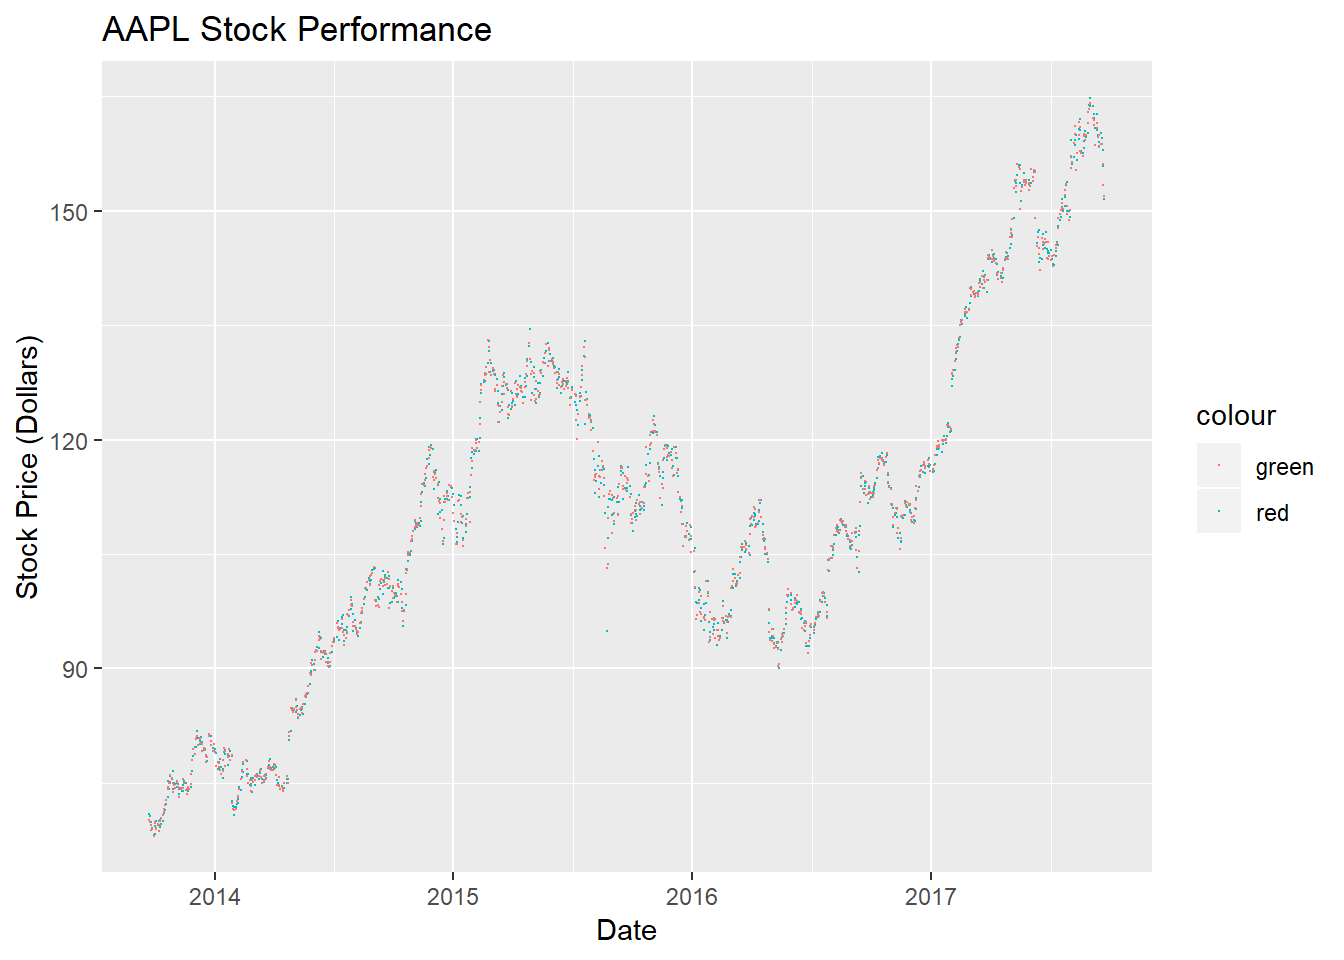
\includegraphics{FinalReport_files/figure-latex/unnamed-chunk-2-1.pdf}

We see here that often when the stock dips, that it rebound within a day
or so. This is a bit misleading because we are looking at the stocks on
a day by day timeframe. However, the market reacts much faster and even
the times that it dips and rebounds, traders can make money.

\hypertarget{table-of-percent-change-number-of-days-below-the-moving-average-and-the-percent-change-per-day}{%
\subparagraph{Table of Percent Change, Number of Days Below the Moving
Average, and the Percent Change per
Day}\label{table-of-percent-change-number-of-days-below-the-moving-average-and-the-percent-change-per-day}}

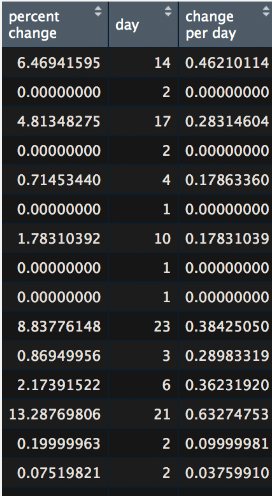
\includegraphics{BBandTable.png}

We also see that there are dips that are pretty significant. The largest
dip was 13\% as well as numerous other dips greater than 1\%. This may
not seem like a lot, but it is significicant given that banks often only
give fractions of a percent in interest. Here we found that the mean
percenage is 2.45\% which is much greater.

Paired with the fact that traders can make moeny on the dips that have a
good rebound, it is safe to say that Bollinger Bands work. Thus having
them would be useful, and usrers should explore other trading platforms
that allow them to use technical indicators.

\hypertarget{comparing-company-performance-to-changes-in-stock-price}{%
\subsubsection{Comparing Company Performance to Changes in Stock
Price}\label{comparing-company-performance-to-changes-in-stock-price}}

I imported a dataset from
\href{https://www.kaggle.com/dgawlik/nyse/version/3\#}{Kaggle} that
shows details about companies listed on the NYSE. I wanted to use this
data set to find a correlation between the information from the data set
and the change in price of a company's stock. I spent some time cleaning
the data set and changing some strings to dates. I also added a row with
the date each measurement was taken, since that information was
originally in the index. I also added a new row that gave the date 1
year after the measurement was taken. I did this so I could easily
access it later when telling the quantmod package what period to get
information from.

I created a function that takes an input of a stock symbol and returns
the associated rows from the dataset along with the change in stock
price over the year after each data point in the set was taken. I made
this function to simplify the process of obtaining data for multiple
company stocks.

During my initial test of this function, I ran into some issues with
errors coming from a few different inconsistencies within the data set,
partly due to some measurements being taken on weekends, when stock
price information is not available. Dealing with all of these issues
would have been very difficult, so I opted instead to simply filter out
the companies whose data contained inconsistencies. Overall, I had to
get rid of data from 165 different companies. However, I kept the data
from 283 companies, and each company provided 4 data points to compare
to, so I believe I still had a large enough data set to gather some
useful information.

I used the LEAPS package and forward subset selection to determine which
5 variables had the biggest effect on the stock's performance the next
year. The top 5 variables were: 1) Fixed Assets 2) Changes In
Inventories 3) Effect of Exchange Rate 4) General and Admin Sales 5) Net
Income

\hypertarget{plots-of-performance-index-vs-stock-price}{%
\subparagraph{Plots of Performance Index vs Stock
Price}\label{plots-of-performance-index-vs-stock-price}}

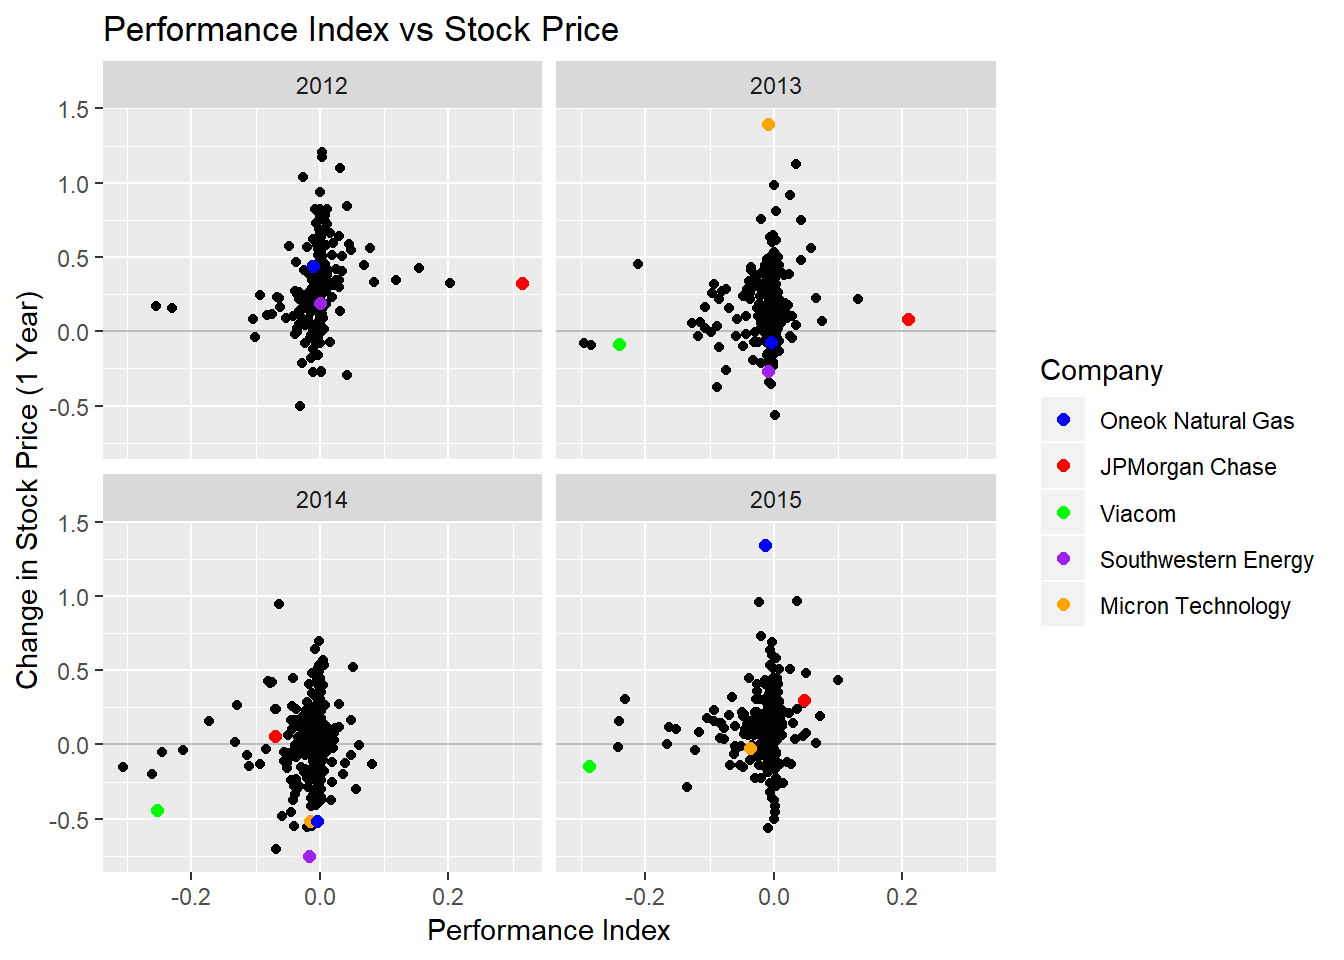
\includegraphics{performance.png}

I created a new variable which is a linear combination of the five most
important variables above, and called it the `Performance Index'. I then
plotted the Performance Index against the change in stock price over the
next year. It looks a bit messy at first, but I think there is quite a
bit of useful information we can get from these graphs.

First, notice that there are many companies grouped around the center of
the x-axis that tend to vary a lot on the y-axis. Smaller companies will
tend to fall in this area, since they don't have large amounts of profit
or loss that would change their performance index by a great amount.
They have the highest variance on the y-axis because it would be easier
for a small company to double in price than it would be for a large
company.

Also note that the companies with exceptionally high or low performance
indexes tend to not vary as much in stock price. This makes sense,
because a large company with an expensive stock won't be likely to
double in price or drop by a large percentage.

I also spent some time looking at the outliers to see if I could
pinpoint a specific reason for the change in stock price or performance
index. I highlighted some noteable companies and explored this question
in the presentation. It is safe to say that having access to more in
depth company data is useful when deciding whether to invest.
Consequently, having the information on your trading platform would be a
big advantage.

\hypertarget{predicting-a-future-stock-price}{%
\subsubsection{Predicting A Future Stock
Price}\label{predicting-a-future-stock-price}}

There are a lot of factors that contribute the price of a stock and how
it moves. Given the growing popularity of algorithmic apps such as
Betterment, I wanted to see if it was possible to predict the price the
future price of a stock.

This results would allow users to decide for themselves as to whether or
not they want to invest their money on a platform that is not traded by
humans.

I decided to test my hypothesis on the S\&P500 because it is a
generalization for many stocks. I also, checked that it had an overall
positive trend, and that overall the stock was increasing.

\begin{Shaded}
\begin{Highlighting}[]
\CommentTok{#Getting the required libraries, we are assuming you already have them installed }
\CommentTok{#If not you can install them from the CRAN using packages.install(<library name>)}
\KeywordTok{library}\NormalTok{(}\StringTok{'quantmod'}\NormalTok{)}
\KeywordTok{library}\NormalTok{(tidyquant)}
\KeywordTok{library}\NormalTok{(}\StringTok{'forecast'}\NormalTok{)}
\KeywordTok{library}\NormalTok{(}\StringTok{'ggplot2'}\NormalTok{)}

\KeywordTok{getSymbols}\NormalTok{(}\StringTok{"SPY"}\NormalTok{, }\DataTypeTok{src=}\StringTok{"yahoo"}\NormalTok{, }\DataTypeTok{from=}\StringTok{"2019-01-01"}\NormalTok{, }\DataTypeTok{to=}\StringTok{"2019-04-27"}\NormalTok{)}
\end{Highlighting}
\end{Shaded}

\begin{verbatim}
## [1] "SPY"
\end{verbatim}

\begin{Shaded}
\begin{Highlighting}[]
\NormalTok{Returns <-}\StringTok{ }\KeywordTok{diff}\NormalTok{(SPY}\OperatorTok{$}\NormalTok{SPY.Close)}\OperatorTok{/}\KeywordTok{lag}\NormalTok{(SPY}\OperatorTok{$}\NormalTok{SPY.Close, }\DataTypeTok{k=}\DecValTok{1}\NormalTok{)}\OperatorTok{*}\DecValTok{1000}
\NormalTok{Returns<-}\KeywordTok{fortify}\NormalTok{(Returns)}

\KeywordTok{ggplot}\NormalTok{(Returns, }\KeywordTok{aes}\NormalTok{(}\DataTypeTok{x=}\NormalTok{SPY.Close) )}\OperatorTok{+}
\StringTok{  }\KeywordTok{geom_histogram}\NormalTok{(}\DataTypeTok{binwidth =} \DecValTok{2}\NormalTok{, }\DataTypeTok{color=}\StringTok{"black"}\NormalTok{,}\DataTypeTok{fill=}\StringTok{"white"}\NormalTok{,}\DataTypeTok{center=}\DecValTok{0}\NormalTok{)}\OperatorTok{+}\StringTok{ }
\StringTok{  }\KeywordTok{scale_x_continuous}\NormalTok{(}\DataTypeTok{breaks=}\KeywordTok{seq}\NormalTok{(}\OperatorTok{-}\DecValTok{26}\NormalTok{, }\DecValTok{36}\NormalTok{, }\DecValTok{2}\NormalTok{))}\OperatorTok{+}
\StringTok{  }\KeywordTok{geom_vline}\NormalTok{(}\DataTypeTok{xintercept =} \DecValTok{0}\NormalTok{, }\DataTypeTok{col =} \StringTok{'darkred'}\NormalTok{)}\OperatorTok{+}
\StringTok{  }\KeywordTok{scale_y_continuous}\NormalTok{(}\DataTypeTok{breaks=}\KeywordTok{seq}\NormalTok{(}\OperatorTok{-}\DecValTok{1}\NormalTok{, }\DecValTok{18}\NormalTok{, }\DecValTok{2}\NormalTok{))}\OperatorTok{+}
\StringTok{  }\KeywordTok{ggtitle}\NormalTok{(}\StringTok{"Frequency of Daily Percentage Change"}\NormalTok{)}\OperatorTok{+}
\StringTok{  }\KeywordTok{xlab}\NormalTok{(}\StringTok{"Percentage Difference"}\NormalTok{)}\OperatorTok{+}
\StringTok{  }\KeywordTok{ylab}\NormalTok{(}\StringTok{"Number of Occurances"}\NormalTok{)}
\end{Highlighting}
\end{Shaded}

\includegraphics{FinalReport_files/figure-latex/unnamed-chunk-3-1.pdf}

We see that the percent change is pretty normally distributed and has
slightly more days where it increases in prices vs when it decreases.

To model it, I chose to use the ARIMA model as the basis for my
prediction. I did so because it is widely used to predict time based
values.

The ARIMA Model is the AutoRegressive Moving Average. Meaning that it
checks how much it correlates with itself, is based off of the moving
average, and uses differencing to make the data stationary. I used 1
degree of differencing, meaning that instead of looking at the price of
the stock, we looked at the difference in price relative to the previous
day.

I modeled the price of the stock using only data from this year because
it would be the most relevant. I chose to use the auto arima function
because it tries all of the ARIMA models and choses the best fit for our
data.

I then used the forecast package in R to try to estimate the price based
on the modeled data.

\begin{Shaded}
\begin{Highlighting}[]
\NormalTok{arimaData <-}\StringTok{ }\KeywordTok{auto.arima}\NormalTok{(SPY}\OperatorTok{$}\NormalTok{SPY.Close)}
\NormalTok{fit.forecast <-}\StringTok{ }\KeywordTok{forecast}\NormalTok{(arimaData)}
\NormalTok{fit.forecast}
\end{Highlighting}
\end{Shaded}

\begin{verbatim}
##    Point Forecast    Lo 80    Hi 80    Lo 95    Hi 95
## 81       293.8294 291.2803 296.3786 289.9308 297.7280
## 82       294.3889 291.1903 297.5874 289.4971 299.2806
## 83       294.9483 291.2116 298.6851 289.2335 300.6632
## 84       295.5078 291.3011 299.7144 289.0743 301.9413
## 85       296.0672 291.4382 300.6963 288.9877 303.1468
## 86       296.6267 291.6106 301.6428 288.9553 304.2981
## 87       297.1862 291.8109 302.5614 288.9654 305.4069
## 88       297.7456 292.0337 303.4575 289.0100 306.4812
## 89       298.3051 292.2753 304.3349 289.0833 307.5269
## 90       298.8645 292.5328 305.1963 289.1809 308.5481
\end{verbatim}

In 2019 there were 80 trading days from January 1st to April 27th that
we were able to use. The first 19 days were used to establish the moving
average. With this data, we were able to predict that the price on the
81st day (April 29th) would be \$293.83 at close.

The actual closing value of the stock was \$293.87. As you can see, our
prediction was very accurate. Often small differences of a few cents can
be attributed to the platform that is gathering the data. Many stock
trading platforms will be within a few cents of each other and the
difference ussually comes down to the speed of their order execution and
what their last reported bid and offer were.

With the success of our model, I would say that it is worth looking more
into the effectiveness of algorithmic trading, perhaps with more stocks.
We have seen that the algorithms can be effective, and if used on a
larger scale, could be profitable.

\hypertarget{our-conclusion}{%
\subsubsection{\texorpdfstring{\textbf{Our
Conclusion}}{Our Conclusion}}\label{our-conclusion}}

Our research was mainly to satisfy curiosity. We wanted to explore what
merits there might be to taking different approaches when going about
the stock market. We advise the reader to take our analysis and
exploration as a starting point to make their own decisions. The stock
market is very complex and there is a reason why so many people have
lost a lot of money in it. Any one who tells you that they have it
figured it out, is lying. Even Warren Buffet lost \$4 billion in a
matter of hours earlier this year. There are a lot more questions that
can be answered, and we hope this provides an idea of how to go about
satisfying your curiosity.

\hypertarget{our-sources}{%
\subsubsection{\texorpdfstring{\textbf{Our
Sources}}{Our Sources}}\label{our-sources}}

\url{https://boeing.mediaroom.com/2018-02-05-Boeing-Debuts-First-737-MAX-7}

\url{https://boeing.mediaroom.com/2018-04-24-Boeing-Ryanair-Announce-Order-for-25-737-MAX-8s}

\url{https://www.cnbc.com/2018/11/20/boeing-shares-fall-after-cancelling-conference-call-on-737-issues.html}

\url{https://www.defensenews.com/land/2018/12/26/heres-the-first-look-at-the-sikorsky-boeing-defiant-helicopter/}

\url{https://cointelegraph.com/news/following-crypto-mining-crash-gpu-producer-nvidia-worst-performer-in-sp-500}

\url{http://rstudio-pubs-static.s3.amazonaws.com/265813_dab79c8eb62d41e381a7e230465573ab.html}

\url{http://rstudio-pubs-static.s3.amazonaws.com/265813_dab79c8eb62d41e381a7e230465573ab.html}

\url{https://www.fool.com/investing/general/2014/01/13/how-micron-technology-plans-to-improve-top-line.aspx}

\url{https://dealbook.nytimes.com/2014/03/19/jpmorgan-to-sell-commodities-unit-for-3-5-billion/}

\url{https://stateimpact.npr.org/pennsylvania/2018/06/11/court-rejects-fracking-companys-appeal-in-rule-of-capture-decision/}

\url{https://cran.r-project.org/web/packages/tidyquant/vignettes/TQ04-charting-with-tidyquant.html}

\url{https://cran.r-project.org/web/packages/quantmod/index.html}

Data Science Cookbook By YuWei Chiu

\hypertarget{reflections}{%
\subsubsection{\texorpdfstring{\textbf{Reflections}}{Reflections}}\label{reflections}}

\hypertarget{alex}{%
\paragraph{Alex}\label{alex}}

I worked on the Bollinger Bands and Stock Prediction portions of the
project. I also found the dataset and was the one who spoke with Dr Dai
about getting the project approved. I coordinated our team meetings and
efforts as well. I wanted to go more in depth with the analysis, but
given that we had homeworks and labs up until the presentation was not
able to. I also wanted to go more in depth in the presentation, as not
everyone has the same financial background. However, I was not able to
due to the time constraint.

\hypertarget{blake}{%
\paragraph{Blake}\label{blake}}

I compared significant publicized events directly related to the
aviation industry to Boeing and Airbus stock prices. My contribution
included all related plots and the written interpretation of the plots.
I also created the SPY plot demonstrating Bollinger Bands and Simple
Moving Average.

\hypertarget{sam}{%
\paragraph{Sam}\label{sam}}

I contributed by analyzing the connection between company performance
and change in stock price. I'm typically not a great public speaker, so
I relied on my teammates to do well in the presentation. Because of
this, I wanted my analysis to be very interesting. I decided to go with
the correlation between company performance and stock price because it's
a simple concept that most people can understand, but it's still a
complex topic that has many avenues for analysis.

\hypertarget{tim}{%
\paragraph{Tim}\label{tim}}

My contribution to the project was the comparison between Nvidia and
AMD. It wasn't the most in-depth or difficult analysis, but I was able
to graph the stock prices for each company over time. Then, since I had
prior knowledge of the Bitcoin blowup and the effect it had on Nvidia
GPUs, I decided to look into what happened to each companies stocks over
that specific timeframe. I actually found pretty much exactly what I
expected - there was a very noticiable impact on both companies
performances on the market.

Since we didn't have any more time, both in the presentation and just in
the class itself, I wasn't able to take the exploration much further.
However, I do find the plenty interesting, and I think that I will look
into stuff like this more in my own time later.


\end{document}
